\documentclass[a4paper,11pt]{article}

\usepackage[margin=2cm]{geometry}
\usepackage{graphicx}
\usepackage{booktabs}
\usepackage{caption}
\usepackage{mathptmx}
\usepackage{amssymb}
\usepackage{amsfonts}
\usepackage{threeparttable}
\usepackage{placeins}
\usepackage{siunitx}
\usepackage{amsmath}
\usepackage[super]{nth}

\sisetup{
    round-mode = figures,
    round-precision = 4
}

\begin{document}

\title{\Large{\textbf{An Unknown Signal}}}
\author{Elan Virtucio}
\date{}
\maketitle

\section{Introduction}
It is very useful to be able to model a given set of data points to an
appropriate degree of accuracy. This can allow for predictions to be made
for an output given some input.
\\ \\
In this instance, a set of data points is given which follows an unknown
signal. The task given was to reconstruct this signal and alongside it,
calculate the sum squared error or residual sum of squares (RSS) to give an
idea of how well the model represents the data.  There are different segments
of this signal and each one can be modelled by either a linear function, a
polynomial function of a fixed degree or some other non-linear function that is unknown.
\\ \\
Although it's possible to model a set of data, ultimately, the results will
be highly dependent on the accuracy and correlation of the data and therefore
problems may arise such as overfitting. The aims of this project were to
minimise these effects and address the limitiations of modelling a data set.

\section{Implementation}
The program is \textit{lsr.py} and it takes in Comma Separated Value (CSV) files
consisiting two columns for the x and y data points respectively. The files can
contain one or multiple line segements and each line segments consists of 20
data points. The segments are split up and for each one, a model is fitted
and it's RSS is calculated. The RSS of each line segment are summed up to
produce the total RSS.
\\ \\
The regression method used was the matrix form of the Least Squares Regression (LSR)
and to account for any form of overfitting, the use of a $k$-fold cross-validation (CV)
was used. There are two implementation that can be used, a fixed $k$-fold
or a random $k$-fold. For example, if $k = 5$, in a fixed $k$-fold, the parts are split up
like so; $[[0, 1, 2, 3], [4, 6, 7, 8], \dots, [16, 17, 18, 19]]$, where the
numbers represent the index of the data point. Whereas, in a random $k$-fold, the parts
can be split up like so; $[[8, 3, 19, 7], [10, 2, 14, 4], \dots, [15, 1, 0, 8]]$,
and this can differ per run. 
\\ \\
The program iterates through a list of defined models as described in
\textit{Table \ref{tab:models}} where $\hat{y}$ is the resulting regression function. These
models are a list object of their own and contains the properties that'll allow it
to model a data set using LSR. These properties are it's name, the relevant function required
to extend the $X$ vector with the relevant feature vectors; where $X$ consists of the x
data points, and additionally, the equation to use. The data is modelled using
each of these models and the RSS is calculated for each one; or to be more precise,
the CV error, which corresponds to the average RSS value that was calculated
during the CV process.  The model that produced the minimum error gets chosen
as the model to use for that data set.

\begin{table}[ht!]
    \centering
    \begin{threeparttable}
    \caption{Models}
    \label{tab:models}
    \begin{tabular}{l c c}
        \toprule
        Name & $X$ & $\hat{y}$ \\
        \midrule
        Linear
            & $\begin{bmatrix}
                1      & x_0       \\
                \vdots & \vdots    \\
                1      & x_{N - 1} 
               \end{bmatrix}$
            & $a_0 + a_1x_i$
            \\ \\
        \nth{2} to \nth{10} Degree Polynomials
            & $\begin{bmatrix}
                1      & x_0       & \dots  & x_0^d       \\
                \vdots & \vdots    & \ddots & \vdots      \\
                1      & x_{N - 1} & \dots  & x_{N - 1}^d
                \end{bmatrix}$
            & $a_0 + a_1x_i + \dots + a_dx_i^d$
            \\ \\
        Exponential
            & $\begin{bmatrix}
                1      & e^{x_0}       \\
                \vdots & \vdots        \\
                1      & e^{x_{N - 1}}
               \end{bmatrix}$
            & $a_0 + a_1e^{x_i}$
            \\ \\
        Sinusoidal
            & $\begin{bmatrix}
                1      & sin(x_0)       \\
                \vdots & \vdots         \\
                1      & sin(x_{N - 1}) 
               \end{bmatrix}$
            & $a_0 + a_1sin(x_i)$
            \\ \\
        Cosinusoidal
            & $\begin{bmatrix}
                1      & cos(x_0)       \\
                \vdots & \vdots         \\
                1      & cos(x_{N - 1})
               \end{bmatrix}$
            & $a_0 + a_1cos(x_i)$
            \\ \\
        \bottomrule
    \end{tabular}
    \begin{tablenotes}
        \item[1] $N =$ \textit{number of data points} $\ \therefore \  N = 20$.
        \\
        \item[2] $a_j \in A = (X^T X)^{-1}X^TY \ \mid \  Y = \begin{bmatrix}y_0 \\ \vdots \\ y_{N - 1}\end{bmatrix}$ 
        \\
        \item[3] $d \in \mathbb{N} \ \mid \ 2 \ \leq \  d \  \leq \  10$
        \\
        \item[4] $i \in \mathbb{Z} \ \mid \ 0 \ \leq \  i \  < \  N$
    \end{tablenotes}
    \end{threeparttable}
\end{table}

\FloatBarrier
    \subsection{Running the Program}
    \textit{lsr.py} takes in CSV files as arguments. There are other optional
    arguments that can be passed: \texttt{--plot} shows a visual plot of the
    fitted line, \texttt{-k=10} uses 10 as the value for k in the $k$-fold CV process,
    \texttt{-v} makes the output more verbose by outputting the model that was
    used per line segment, \texttt{--random-$k$-fold} uses the random implementation
    of $k$-fold CV, \texttt{--no-cross-validation} runs the program without using CV.

\section{Results}
The following results that will be mentioned were obtained using the lab machines.
There were multiple different runs of the program accross all of the train data
files that were provided. This included changing the $k$-fold CV methods used including
changing the $k$ values as well running it without CV. With these runs, it was
surmised that the three function types that were used were linear, cubic and sinusoidal.
This was because across all of the basic train files provided, these were the models
that the program fitted consistently and additionally, they visually produced
acceptable plotted fits for the data. The calculated RSS values for the basic training data
files shown in \textit{Table \ref{tab:main_results}} are very small and further validates the fitted
models. There were other models that were fitted with the advance and noise files, however,
considering the specification of the project of having only a linear, a polynomial of a
fixed degree, or some additional non-linear function in the line segments, these were
ruled out as cases of overfitting.
\\ \\
These redundant models were then commented out for future runs of the program
and therefore were not part of the iteration of the list of models to fit the data
in. An instance of this is shown in \textit{Table \ref{tab:main_results}}.

\begin{table}[ht!]
    \scriptsize
    \centering
    \caption{Results of training data files using a fixed $k$-fold CV where $k = \{5, 10, 20\}$}
    \label{tab:main_results}
    \begin{tabular}{l l l}
        \toprule
        File (.csv) & RSS & Fitted Models \textit{w.r.t.} the Line Segments \\
        \midrule
        basic\_1
            & \num{2.22853205725e-27}
            & Linear
        \\
        basic\_2
            & \num{2.0549826581e-27}
            & Linear, Linear
        \\
        basic\_3
            & \num{3.80497072739e-18}
            & Cubic
        \\
        basic\_4
            & \num{8.64481149963e-11}
            & Linear, Cubic
        \\
        basic\_5
            & \num{2.15680882375e-25}
            & Sinusoidal
        \\
        adv\_1
            & \num{220.445220441}
            & Sinusoidal, Linear, Cubic
        \\
        adv\_2
            & \num{3.68513205045}
            & Sinusoidal, Linear, Sine
        \\
        adv\_3
            & \num{1019.02994947}
            & Sinusoidal, Cubic, Sinusoidal, Linear, Sinusoidal, Cubic
        \\
        noise\_1
            & \num{12.2074601401}
            & Linear
        \\
        noise\_2
            & \num{849.552746233}
            & Linear, Cubic
        \\
        noise\_3
            & \num{482.909050785}
            & Linear, Cubic, Sinusoidal
        \\
        \bottomrule
    \end{tabular}
\end{table}
\FloatBarrier

\noindent
\textit{Table \ref{tab:noise_no_cv_results}} and \textit{Figure \ref{fig:noise_1_no_cv}}
shows us an instance of overfitting. It can be discerned that \textit{noise\_1.csv} should
be fitted by a linear model. Although the regression line in \textit{Figure \ref{fig:noise_1_no_cv}}
appears as linear, it was actually based on a cubic function. The noisy results from
\textit{Table \ref{tab:main_results}} shows the effects of how CV can account for
instances of overfitting. Additionally, when comparing the results from
\textit{Table \ref{tab:main_results}} and \textit{Table \ref{tab:noise_no_cv_results}},
the RSS value in the latter showed a lower RSS value than the former result. This
shows an instance of where a lower RSS value doesn't necessarily have to
correspond to an agreeable solution.

\begin{table}[ht!]
    \begin{minipage}{0.5\linewidth}
    \scriptsize
    \centering
    \caption{Results of noise training data files without CV}
    \label{tab:noise_no_cv_results}
    \begin{tabular}{l l l}
        \toprule
        File (.csv) & RSS & Fitted Models \textit{w.r.t.} the Line Segments \\
        \midrule
        noise\_1
            & \num{10.9850554645}
            & Cubic
        \\
        noise\_2
            & \num{797.916656822}
            & Cubic, Cubic
        \\
        noise\_3
            & \num{477.699338119}
            & Cubic, Cubic, Sinusoidal
        \\
        \bottomrule
    \end{tabular}
    \end{minipage}
    \begin{minipage}{0.5\linewidth}
    \centering
    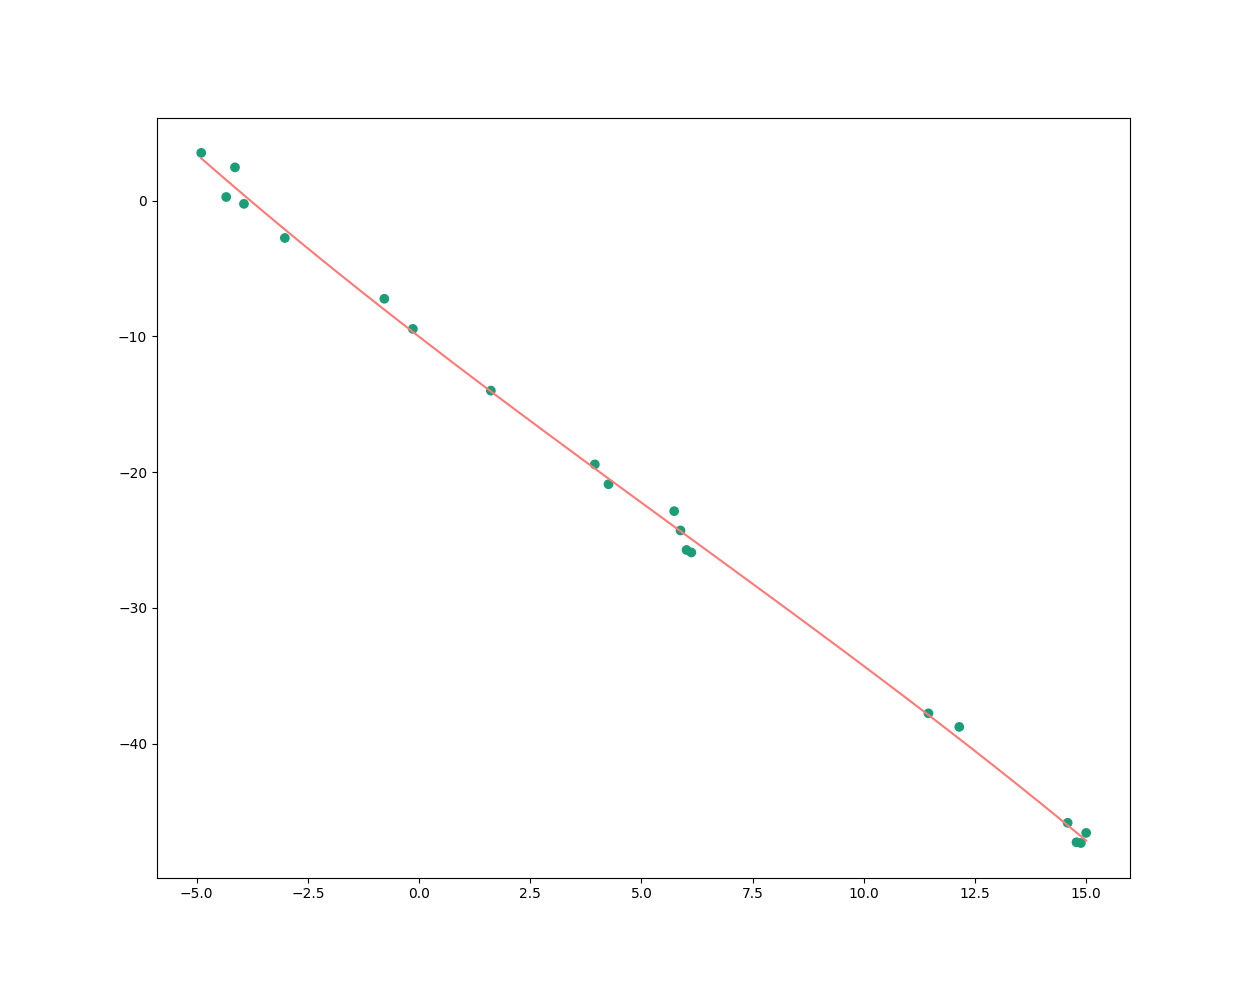
\includegraphics[width=1\linewidth]{res/noise_1_no_cv.png}
    \captionof{figure}{Plot of fitted line of \textit{noise\_1.csv} from \textit{Table \ref{tab:noise_no_cv_results}}}
    \label{fig:noise_1_no_cv}
    \end{minipage}
\end{table}
\FloatBarrier

\noindent
There are different ways of implementing CV and each one may yield different
results. This is because of how the data is split up into training and validation sets
differs per method. Having a validation set of data that is relatively close
to the true data is the ideal but it would be difficult to achieve if the true
data is unknown which should be the standard case for data analysis. The use of
a $k$-fold CV creates a scenario where each data gets a chance to be part of the
validation set and also part of the training set. This creates an average representation
of how well the data should fit a given model.
\\ \\
However, depending on the value of $k$, it can affect the results. This should be the
expectation as depending on the size of the validation set, it'll affect the
variability and bias of the iterations of the $k$-fold CV process. For example, a 20-fold
CV would result in a validation set of size 1 since the size of a line segment is 20.
This instance is also known as leave-one-out CV. In this case, although the intuition is that
CV error produced will be unbiased, it may produce high variability especially in noisy
data. In that sense, finding the optimum value for $k$ as an extra step could lead
to a more agreeable solution. However, trying to find this would be computationally
expensive, especially in the case of larger data sets. Unfortunately, due to
the simplicity and size of the provided data set, the results of
\textit{Table \ref{tab:main_results}} is unable to demonstrate a noticable
difference between appropriate $k$ values to justify this intuition.
\\ \\
The grouping of the data in $k$-fold CV can also affect the solution. A more
agreeable or less agreeable solution can be produced depending which data gets
grouped together. This can be demonstrated using the random implemenation of $k$-fold
CV. The results are shown in \textit{Table \ref{tab:adv_3_random_cv}} and a 5-fold
CV was used as this allowed for sufficient data per set to emphasise the effects of a random
grouping of the data. Due to it's random nature, the solution produced will be
arbitrarily acceptable or not. For \textit{adv\_3.csv}, the intuition was that it should
follow a linear, cubic, sinusoidal, linear, sinusoidal, cubic pattern of fitted models
\textit{w.r.t.} to the line segments as shown in \textit{Figure \ref{fig:adv_3}}.
This was not the result however in \textit{Table \ref{tab:main_results}}.
\\ \\
Using a random $k$-fold CV has yielded different fits of the data including the
desired result but also some results that are worse off such as in the case where
the \nth{4} line segment has overfitted instead, in runs \textit{2, 6, 7} and \textit{9}.
Since it's random, the results may not necassarily be reliable. An alternative
implementation of the random $k$-fold may be more suitable such that it attempts to
create a distribution of the fitted models of based on an arbitrarily large number
of runs and find a solution based on that distribution. However, this is computationally
expensive.  That being said, that method may still not yield the desired result on the
basis that based on \textit{Table \ref{tab:main_results}}, only 2 out of 10 runs yielded
the desired result. Ultimately, the effects of CV is constrained by the data provided.

\begin{table}[ht!]
    \begin{minipage}{0.5\linewidth}
    \scriptsize
    \centering
    \caption{Results of multiple runs of \textit{adv\_3.csv} using a random 5-fold CV}
    \label{tab:adv_3_random_cv}
    \begin{tabular}{l l l}
        \toprule
        Run & RSS & Fitted Models \textit{w.r.t.} the Line Segments \\
        \midrule
        1
            & \num{1020.76902787}
            & Linear, Cubic, Sinusoidal, Linear, Sinusoidal, Cubic
        \\
        2
            & \num{1008.18577729}
            & Linear, Cubic, Sinusoidal, Cubic, Sinusoidal, Cubic
        \\
        3
            & \num{993.507417746}
            & Cubic, Cubic, Sinusoidal, Linear, Sinusoidal, Cubic
        \\
        4
            & \num{1019.02994947}
            & Sinusoidal, Cubic, Sinusoidal, Linear, Sinusoidal, Cubic
        \\
        5
            & \num{1019.02994947}
            & Sinusoidal, Cubic, Sinusoidal, Linear, Sinusoidal, Cubic
        \\
        6
            & \num{1006.4466989}
            & Sinusoidal, Cubic, Sinusoidal, Cubic, Sinusoidal, Cubic
        \\
        7
            & \num{1006.4466989}
            & Sinusoidal, Cubic, Sinusoidal, Cubic, Sinusoidal, Cubic
        \\
        8
            & \num{1020.76902787}
            & Linear, Cubic, Sinusoidal, Linear, Sinusoidal, Cubic
        \\
        9
            & \num{1008.18577729}
            & Linear, Cubic, Sinusoidal, Cubic, Sinusoidal, Cubic
        \\
        10
            & \num{1019.02994947}
            & Sinusoidal, Cubic, Sinusoidal, Linear, Sinusoidal, Cubic
        \\
        \bottomrule
    \end{tabular}
    \end{minipage}
    \begin{minipage}{0.5\linewidth}
    \centering
    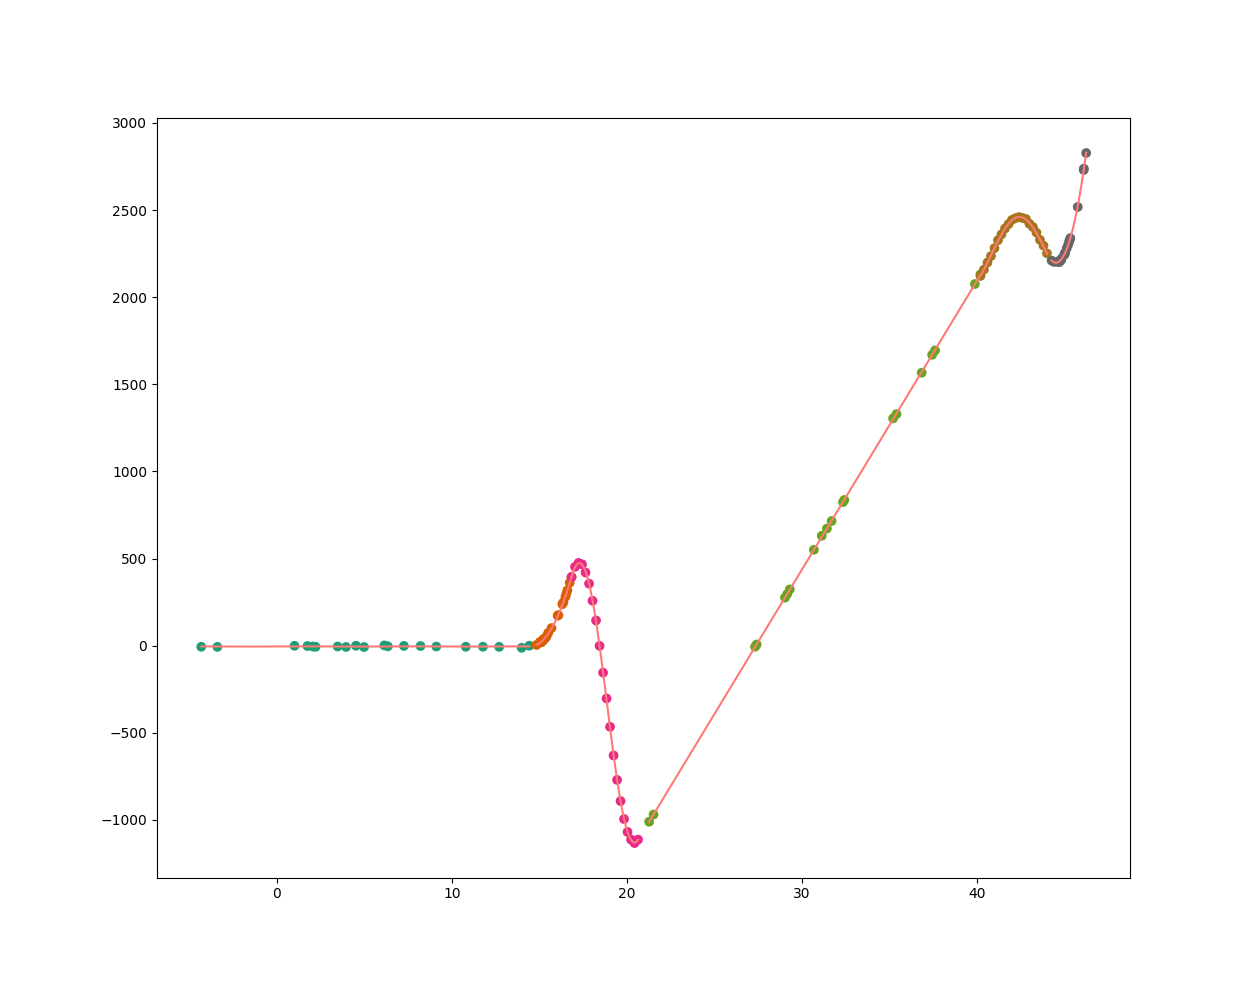
\includegraphics[width=1\linewidth]{res/adv_3.png}
    \captionof{figure}{Plot of fitted line of \textit{adv\_3.csv} from \textit{Table \ref{tab:main_results}}}
    \label{fig:adv_3}
    \end{minipage}
\end{table}
\FloatBarrier

\section{Conclusion}
LSR and CV were sufficient enough to identify the appropriate models to be used
for each line segment. They could have been fitted as a linear, cubic or sinusoidal
model. Cases of overfitting were minimised and accounted for using CV. However,
there were instances where CV was not enough to yield an agreeable solution.
\\ \\
Different methods of CV were able to achieve an agreeable solution and some
produced poorer results. This shows that depending on the data set provided, some
methods may be more preferable than the others. By discerning any patterns of which
method are most appropriate for a data set might be a way of counteracting this.
This includes any imbalances in a data set and also the amount of data provided as
patterns in a data set that could have an effect on how CV is implemented. Another
modification would be to use regularisation along with CV to futher validify a
solution. Lastly, it's also possible that even with these methods, an agreeable
can't be found. These methods are dependent on how well the data represents a
some model to begin with.
\end{document}
